\documentclass[border=3pt,tikz]{standalone}
\usetikzlibrary{intersections,through,shapes,shapes.geometric}
\usetikzlibrary{calc}

% side lengths of triangle
\newcommand{\AB}{5cm}
\newcommand{\AC}{12cm}
\newcommand{\BC}{13cm}

\begin{document}

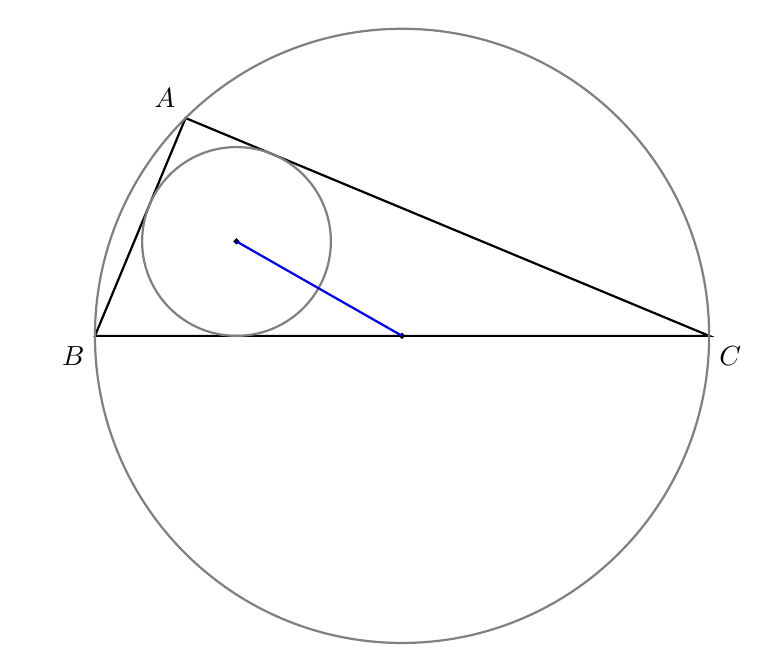
\begin{tikzpicture}[scale=0.6,thick]
  % draw points B and C horizontally (arbitrary choice)
  \coordinate (B) at (0, 0);
  \coordinate (C) at (\BC, 0);

  % get coordinates of A based on position of B and C
  \begin{pgfinterruptboundingbox}% prevent spacing from spilling out
      % draw circle with center B and radius AB
      \node (r1) at (B) [circle through=($ (B) + (0:\AB) $)] {};
      % draw circle with center C and radius AC
      \node (r2) at (C) [circle through=($ (C) + (0:\AC) $)] {};
  \end{pgfinterruptboundingbox}
  % A lies at the intersection of the two circles
  \coordinate (A) at (intersection 2 of r1 and r2);

  % draw triangle ABC
  \draw (B) node[below left] {$B$} 
     -- (C) node[below right] {$C$}
     -- (A) node[above left] {$A$} 
     -- cycle; 
     
  % path of angle bisector at A
  \coordinate (A1) at ($(A)!10cm!(B)$);
  \coordinate (A2) at ($(A)!10cm!(C)$);
  \coordinate (A3) at ($(A1)!0.5!(A2)$); % midpoint of A1-A2
  \path[name path=AA] (A) -- (A3);
%  \draw[name path=AA,blue] (A) -- (A3);

  % path of angle bisector at C
  \coordinate (C1) at ($(C)!15cm!(A)$);
  \coordinate (C2) at ($(C)!15cm!(B)$);
  \coordinate (C3) at ($(C1)!0.5!(C2)$); % midpoint of C1-C2
  \path[name path=CC] (C) -- (C3);
%  \draw[name path=CC,red] (C) -- (C3);
    
  % The center of the circle inscribed in the triangle is located.
  \path[name intersections={of={AA} and {CC}, by={O1}}];
  % mark the center of the inscribed circle
  \draw [fill] (O1) circle (1pt);
  % draw inscribed circle
  \draw [gray]
    let \p1=($ ( $(A)!(O1)!(B)$ )-(O1)$) 
      in (O1) circle ({veclen(\x1,\y1)});

  % mark the center of the circumscribed circle
  \coordinate (O2) at (\BC/2,0);
  \draw [fill] (O2) circle (1pt);
  % draw circumscribed circle
  \draw [gray] (O2) circle (\BC/2);
  
  % connect the two centers
  \draw [blue] (O1) -- (O2); 

\end{tikzpicture}

\end{document}
